\section{Introduction}
This lab assignment aims to use linear control theory to allow the control of a helicopter using a joystick. Trying to control the helicopter, without a regulator to stabilize the system, is nearly impossible. The helicopter becomes hard to control, and will crash if the user makes a small mistake.

\begin{figure}[htb]
	\centering
	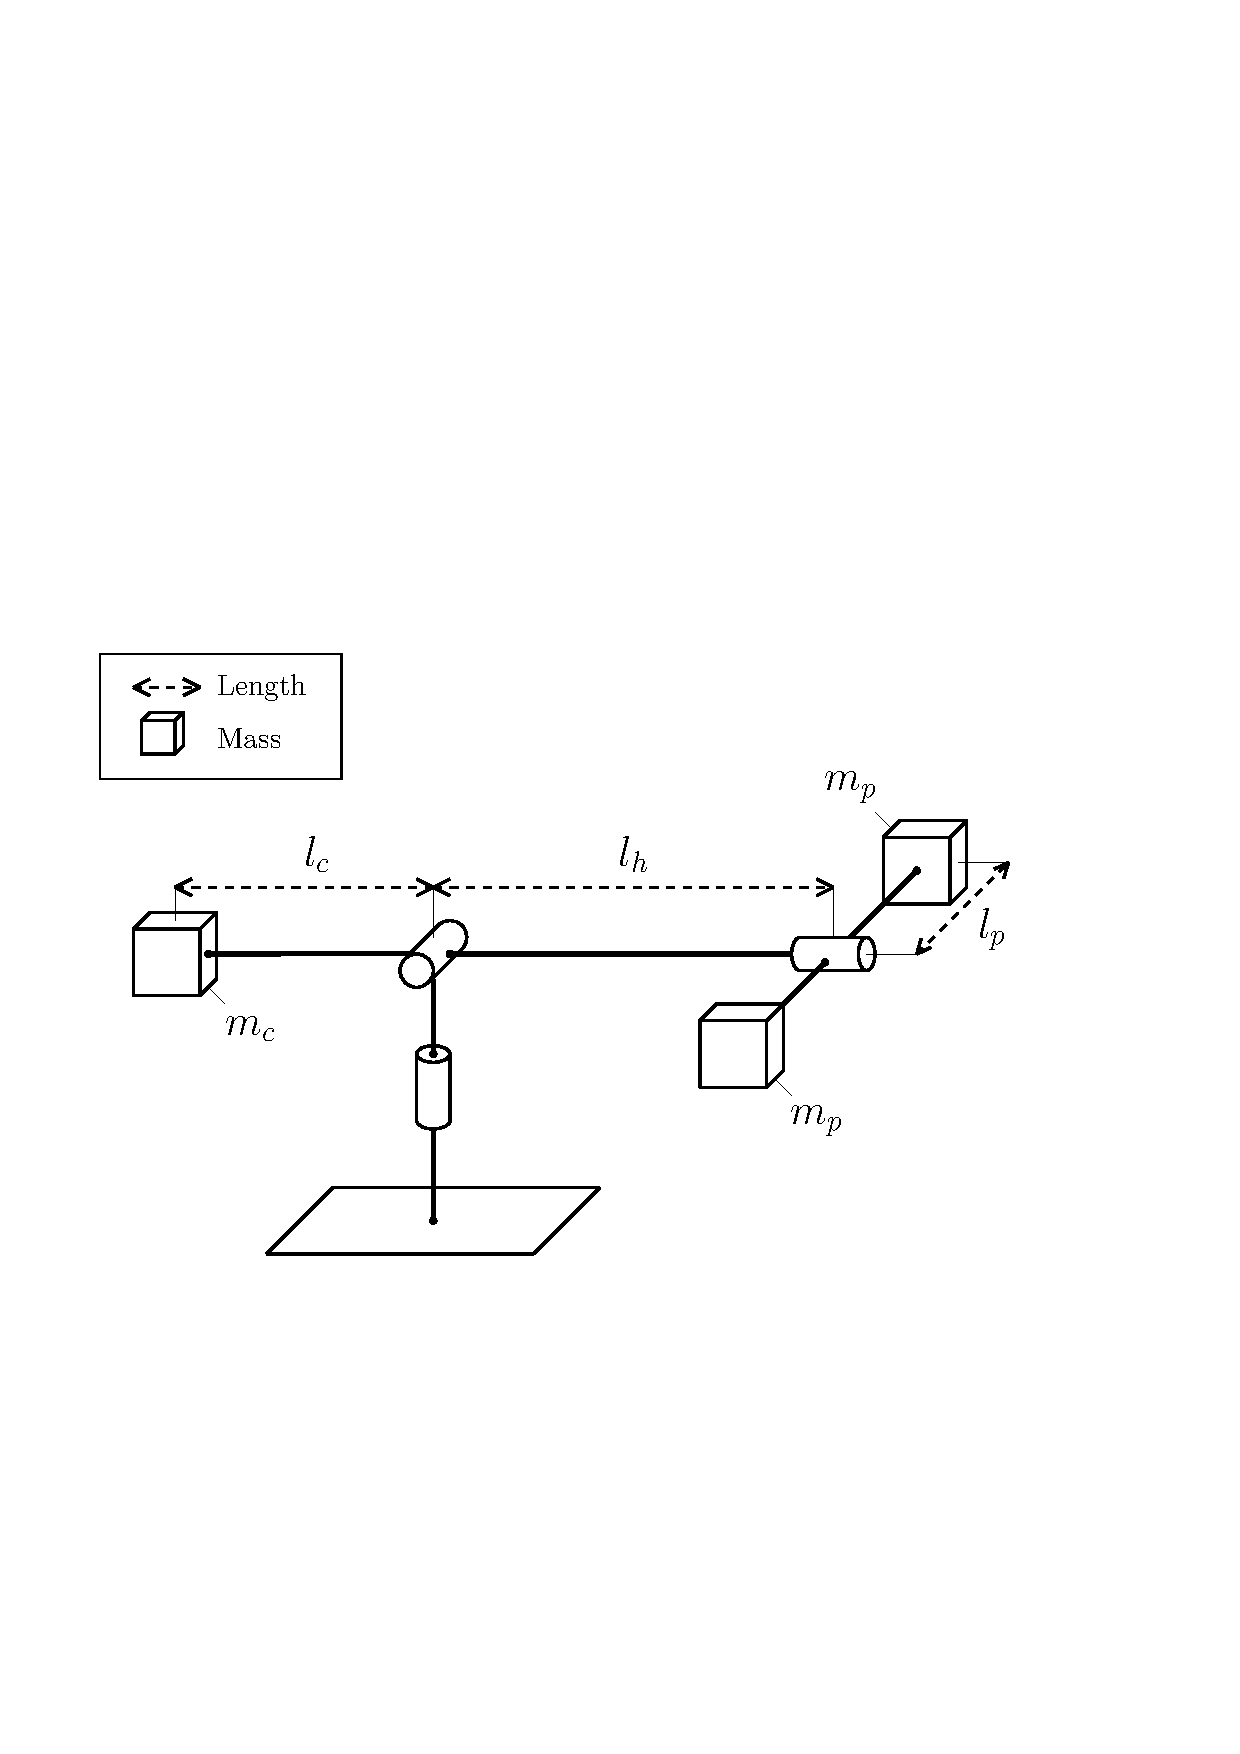
\includegraphics[width=0.9\linewidth]{images/helicopter.pdf}
    \caption{Helicopter setup, \cite{HeliLabAssignment}}
    \label{fig:setup}
\end{figure}


Figure \ref{fig:setup} shows the helicopter setup used in the lab. The 2 propellers are balanced with a counterweight on the other side of the center joint. These are controlled by changing the voltage to each motor. \medskip

To complete the task, we have derived a model for the helicopter system. In the different sub problems of the lab assignment, this model will be used to test different regulators. During the lab, we are testing P, PD and multivariable controllers. In the last part of the lab we will also implement an estimator for the states, and use observability to estimate states that aren't measured. This will be combined with an LQR regulator to control the helicopter. \medskip

This rapport will have two main parts, theory and results. During the theory we will derive all the equations for our model and controllers. The results will showcase the helicopter behaviour, and compare it to other controllers. Here we also discuss why some controllers work better than others.\medskip

Tables with constants and parameters can be found in Appendix \ref{sec:nomenclature}. Appendix \ref{sec:matlab_snippets} contains Matlab code snippets. We used Matlab 2014a in the lab.